\chapter{Simulation}
\label{Sim}
Network simulation is a practical way of developing and researching networks and their
behavior. Especially in WSNs, the main focus is not on one particular sensor node, but on
the behavior of the entire network (which can consist of thousands of sensor nodes). It would
be impractical to do initial research based on real world testing and deployment, as that would cost exorbitant amounts of money, and create logistical nightmares to set up the WSN. For this reason, a valid
simulation tool is a necessity for further studies. This chapter focuses on the simulation; it 
includes discussion about the simulator, simulation and scenario setups and simulation procedure.

\section{TinyOS Simulator - TOSSIM}
\label{Sim:TOSSIM}

The simulator used in this project is called TOSSIM\@. TOSSIM is a discrete, event-driven WSN simulator included in TinyOS. Compiling unchanged TinyOS applications
directly into its framework, TOSSIM can simulate thousands of motes running complete
applications \cite{LLWC}. It fulfils the requirements of being a TinyOS simulator; such requirements include: scalability, completeness and fidelity. TOSSIM is a shared library, therefore a script written with C++ or Python must be created to run the simulation.  Python is chosen in this project as it can dynamically interact with the simulation.
\newline

Configuring networks for TOSSIM simulation usually includes setting
up both a network topology and an interference model. For the topology, a file with the format~\texttt{Source Destination Gain} may be created. TOSSIM uses Closest Pattern Match (CPM) algorithm to calculate the channel noise. It is a wireless noise simulation model
based on statistical extraction from empirical noise data. It takes a noise trace as input to generate the interference model. This method is accepted to be much more accurate and preferable than the traditional, Independent Packet Loss (IPL) models~\cite{TOSSIM}.

\section{Enabling Simulation}
\label{Sim:Enabling}

The simulation has enabled for a multi-hop network with BLIP 1.0 implementation before. The radio stack for this simulation was CC2420. But due to considerable changes that was done in both CC2420 radio stack and BLIP, the re-enable of simulation for BLIP is required. 
\newline

As mentioned in Section \ref{Sim:radio stack}, the rfxlink radio stack unifies CC2420 and RF230. Furthermore, the TOSSIM simulation support for rfxlink has been developed by Morten Tranberg Hansen. But either BLIP 1.0 nor BLIP 2.0 has been implemented on top of rfxlink. In oder to execute simulation, the simulated rfxlink had to be moved underneath BLIP 2.0. 
\newline

The enabling of simulation took the following steps: 
\begin{itemize}
\item Merge into the branch to Morten Tranberg Hansen's rfxsim repository \cite{rfxsim}. 
\newline

\item Add the simulated ``chip driver'' layer - TossimDriverLayerC to the already supported CC2420 and RF230 radio chips. 
\newline

\item Introduced 802.15.4 packets into TOSSIM. TinyOS basic packets abstraction is Active Message (AM), but 6LoWPAN uses 802.15.4 packets. Introduction of 802.15.4 packets into TOSSIM is essential for the simulation to run.
\newline

\item Configure the simulation to support BLIP 2.0. Using short IEEE 802.15.4 address for Ieee154Send interface in IPDispatch. 
\newline

\item The compiler GPP is used to compile BLIP 2.0. At the meanwhile, the 6LoWPAN library is written in C. \texttt{extern ``C''} had to be added to notify the C++ compiler of the C style functions.
\newline

\item Write makefile to include 6LoWPAN object files into simulation library.
\end{itemize}

\section{Simulation Setups}
\label{Sim:Setup}
\subsection{Methodology}
\label{Sim:Method}
The application~\texttt{UDPEcho} is used in the simulation to evaluate the performance of RPL protocol. It is configured to behave similar to the application~\texttt{Ping}. A node sends out a data packet to a node and receives the echo packet from the receiver. The application is installed on both simulated root node and child nodes. In the simulation, the root node will ``ping'' each child 100 times, that is it will send \texttt{UDPEcho} packets 100 times to a child node, then continue to send another 100 \texttt{UDPEcho} packets to the next child node until all children are  ``pinged''.     
\newline

The simulation will be done for various scenarios with different number of nodes, as well as RPL with OF0 and MRHOF respectively. The results of the simulation is visualized with the python plotting library \texttt{Matplotlib}.

\subsection{Simulation Scenarios}
\label{Sim:Scenarios}
\begin{figure}[!ht]
 % \begin{center}
 	\centering
    \leavevmode
    %\framebox{
      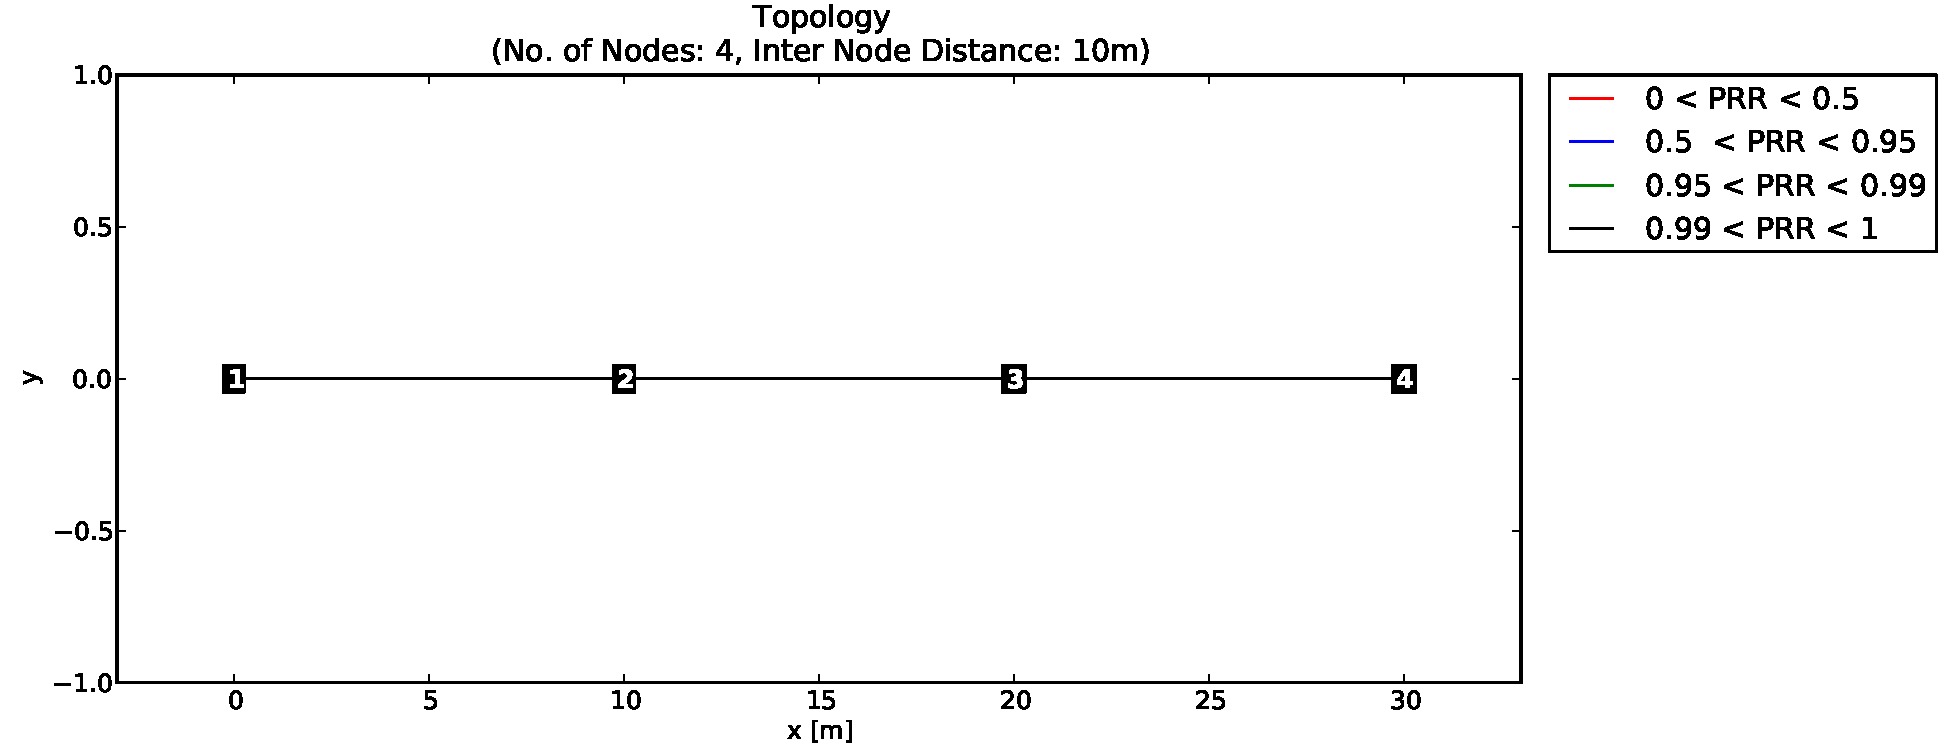
\includegraphics[scale=0.35]{Pics/results/topo4_dist10_line.pdf}
    \caption{Line scenario}
    \label{fig:scenario_line}
 % \end{center}
  	%\vspace{-80pt}	
\end{figure}

\begin{figure}[!ht]	
%  \begin{center}
  	\centering
    \leavevmode
    %\framebox{
      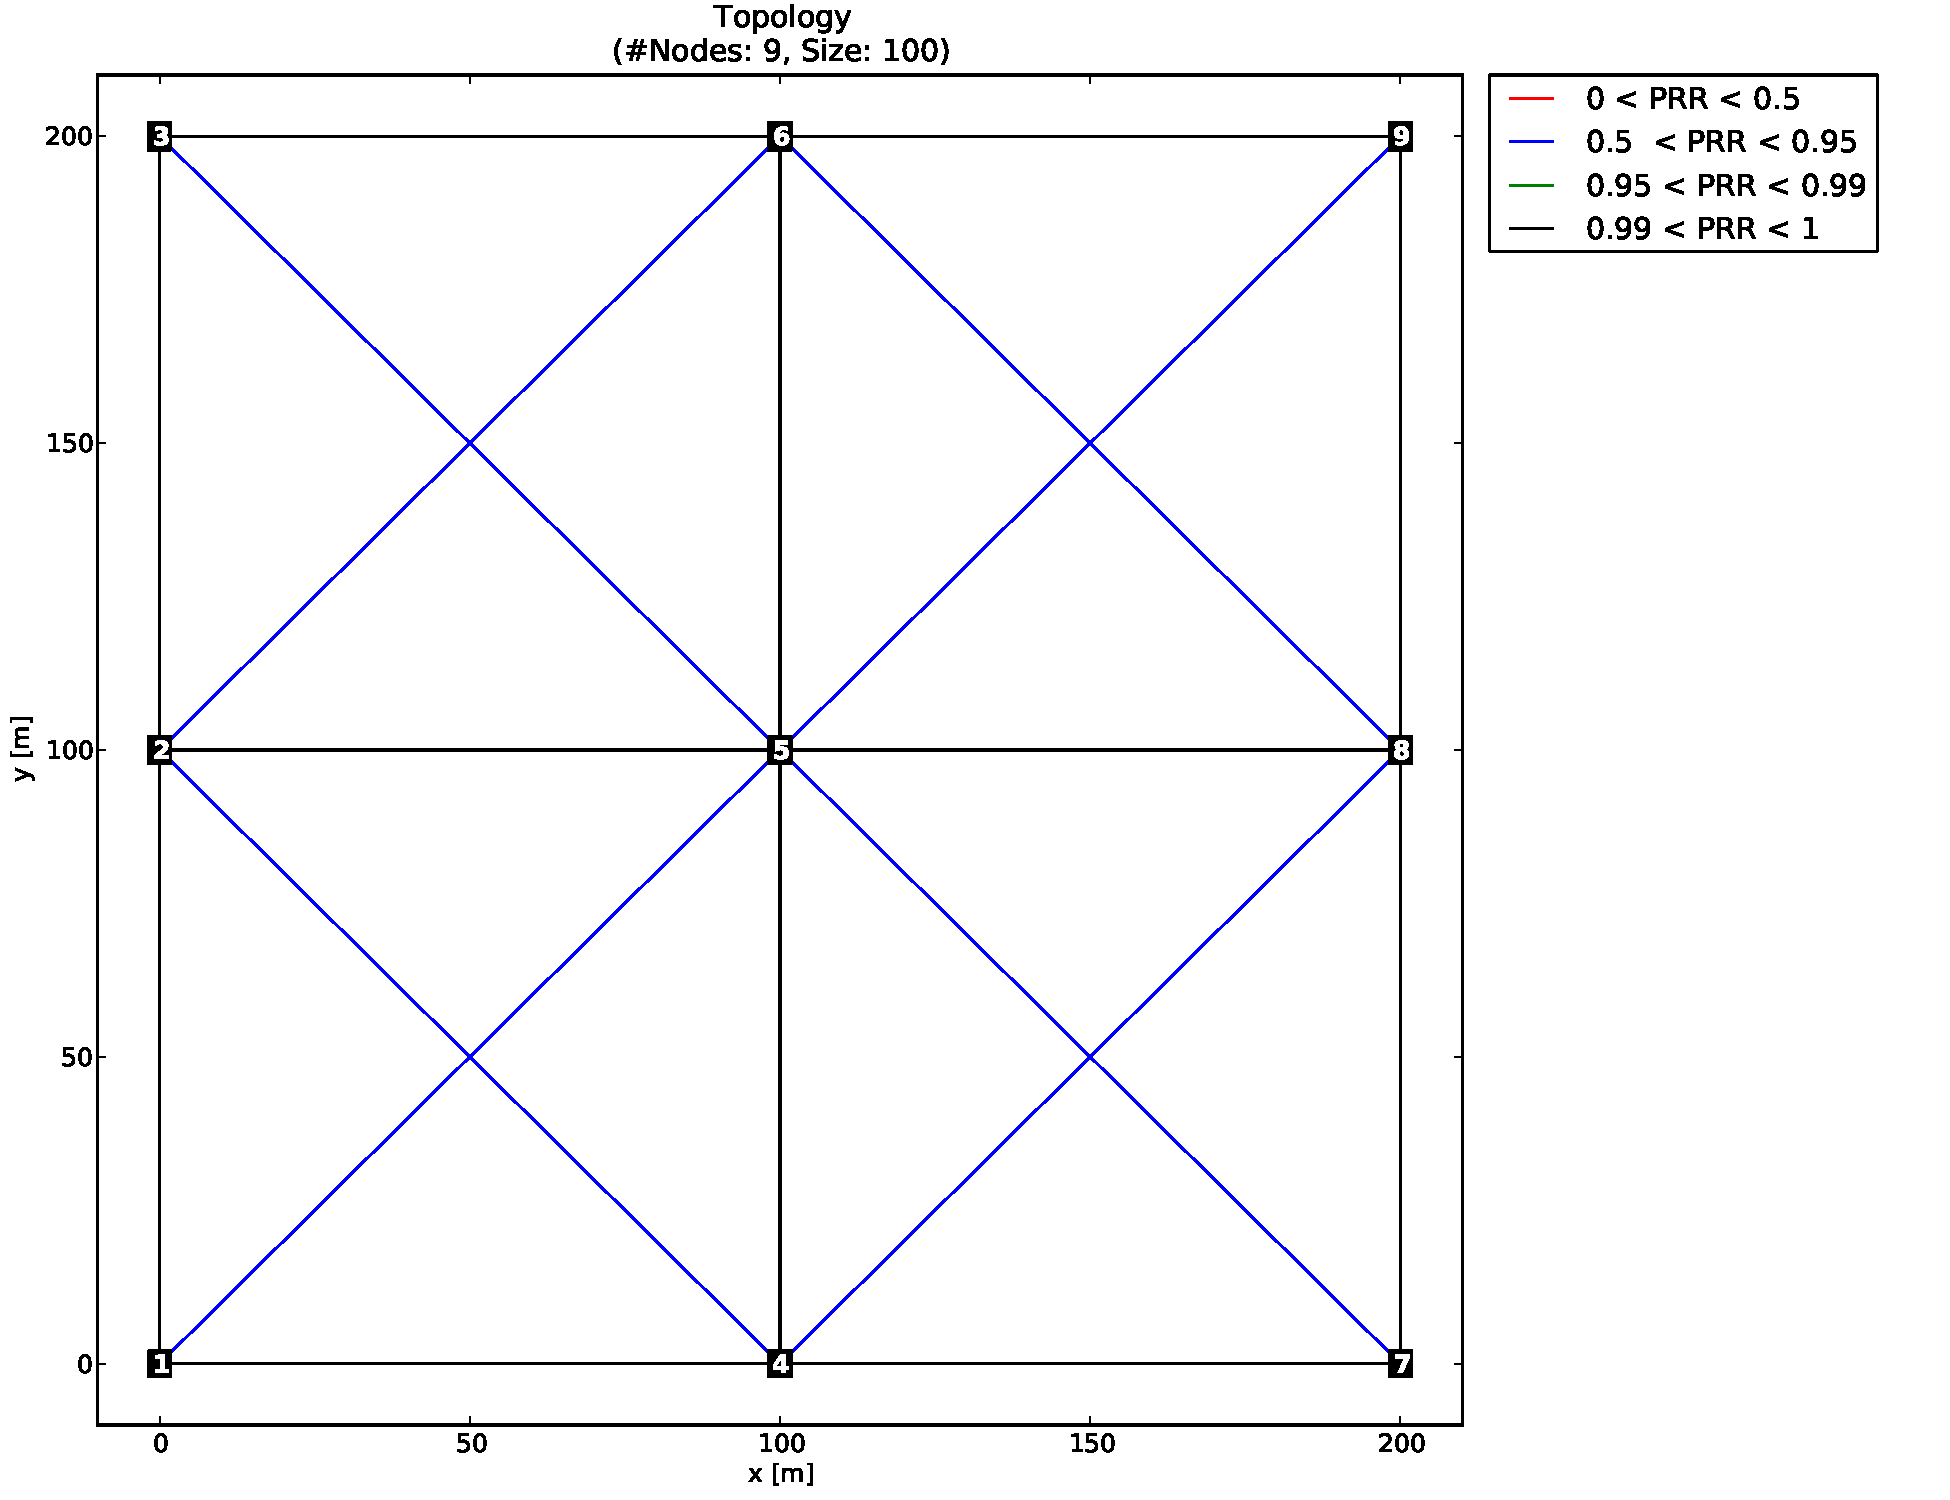
\includegraphics[scale=0.35]{Pics/results/topo9_dist100_grid.pdf}
    \caption{Grid scenario}
    \label{fig:scenario_grid}
%  \end{center}
\end{figure}

Two kinds of scenarios are created for the simulation - a line scenario and a grid scenario. In the line scenario the neighboring nodes are equal distanced; in the grid scenario, the number of nodes should be a square number, and the grids are square grids. Figure \ref{fig:scenario_line} shows a 4 nodes line scenario with 10 m inter node distance. A 9 nodes grid scenario with 100 m inter node distance is shown in Figure \ref{fig:scenario_grid}.
\newline

The Packet Reception Ratio (PRR) is estimated from Signal-to-Noise Ratio (SNR). The estimation is based on the measurement in \cite{RL08}:
\[
PRR = (1-0.5*erfc(\frac{\beta_1*(SNR-\beta_2)}{\sqrt{2}}))^{23*2}
\quad{\beta_1} = 0.9794, {\beta_2} = 2.3851
\] 
with 
\[
SNR = Signal(dBm)- Nosie(dBm) = -(50 + 20 {\log}(Distance)) - (-98)(dBm)
\] 
The relationship between distance and PRR is shown in Figure \ref{fig:prr}. When the distance between two nodes is smaller than 120 meters, they can hear each other with a PRR value of 0.99. Once the distance is larger than 120m, the PRR begins to decline up until it reaches a value of 0, which corresponds to a distance of 165 meters. This means that at a distance of over 165 meters the two nodes are at least 2 hops apart.

\begin{figure}[htbp]
  \begin{center}
    \leavevmode
      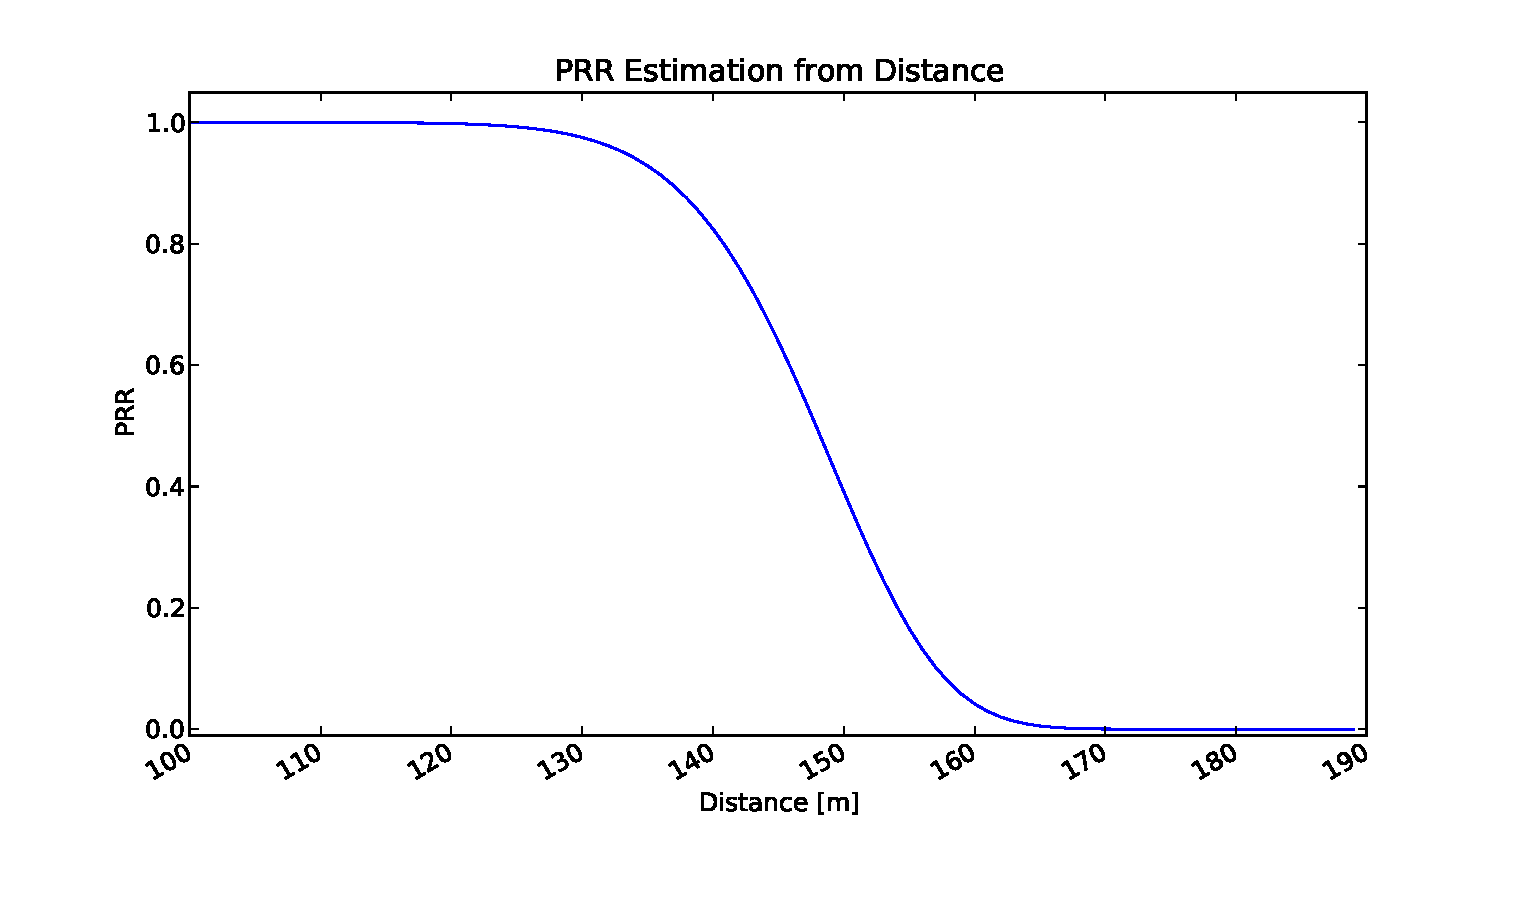
\includegraphics[scale=0.45]{Pics/prr.pdf}
   \caption{Relationship between distance and PRR}
    \label{fig:prr}
  \end{center}
\end{figure}

\subsection{Trickle Parameters and Variables}
\label{trickle parameters}
The Trickle timer parameters and initial variables in the simulation are set as below:
\begin{itemize}
\item Minimum time interval size $Imin = 0$

\item Maximum time interval size $Imax = 256 s$

\item Redundancy constant $K = 255$

\item Initial current interval size $I = 256 ms$

\item Initial timer value t randomly chosen in range $[128, 256) ms$

\item Initial counter $C = 0$
\end{itemize}

\subsection{Simulation Metrics}
\label{Sim:metrics}
The metrics that are used to evaluate the RPL performance are:
\begin{itemize}
\item Mean packet loss over 100 runs: Packet loss rate shows the quality of the links between nodes. A good multi-hop routing protocol should be able to forward packet properly to the destination under the certain link condition. The mean packet loss rate of both OF0 and MRHOF will be compared.
\newline

\item Mean Route Trip Time (RTT) over 100 runs: The mean RTT for various scenarios and both OF0 and MRHOF with link ETX (hereinafter to be shorted as MRHOF) will be evaluated.
\newline

\item Cumulative distribution function (CDF) of time to default route detection: when a node receives the first DIO message from a lower rank node, it sets the default route entry. The sending of the DIO is controlled by Trickle timer. The CDF of default route discovery time will demonstrate the characteristics of the Trickle algorithm.
\newline

\item Mean control message overhead over 100 runs: In order to show the effect of Trickle timer, the amount of ICMP messages a node sends out during time intervals will be shown.
\end{itemize}







